\documentclass{article}

\usepackage[brazilian]{babel}
\usepackage{indentfirst}
\usepackage[T1]{fontenc}
\usepackage[utf8]{inputenc}
\usepackage[hidelinks]{hyperref, xurl} % \url
\usepackage{graphicx} % png

\newfloat{Código}
\captionsetup{Código}

\author{Gabriel G. de Brito}
\title{Implementação simulada da arquitetura Sagui em Bando (vetorial)}

\begin{document}

\maketitle

\section{Introdução}

Esse trabalho apresenta a implementação no simulador Logisim
Evolution\footnote{\url{https://github.com/logisim-evolution/logisim-evolution}}
da arquitetura Sagui em Bando, uma versão vetorial da arquitetura Sagui. A
implementação foi um sucesso e todos os requisitos foram atendidos.

Além disso, o trabalho ressalta as diferenças entre a implementação do Sagui em
Bando em relação à implementação do Sagui entregue como Trabalho I.

\section{O Sagui em Bando}

A figura \ref{sagui} apresenta o diagrama do processador.

\begin{figure}[h]
	\centering
	% 0.9 forces the height to be just right to fit this image in the first page.
	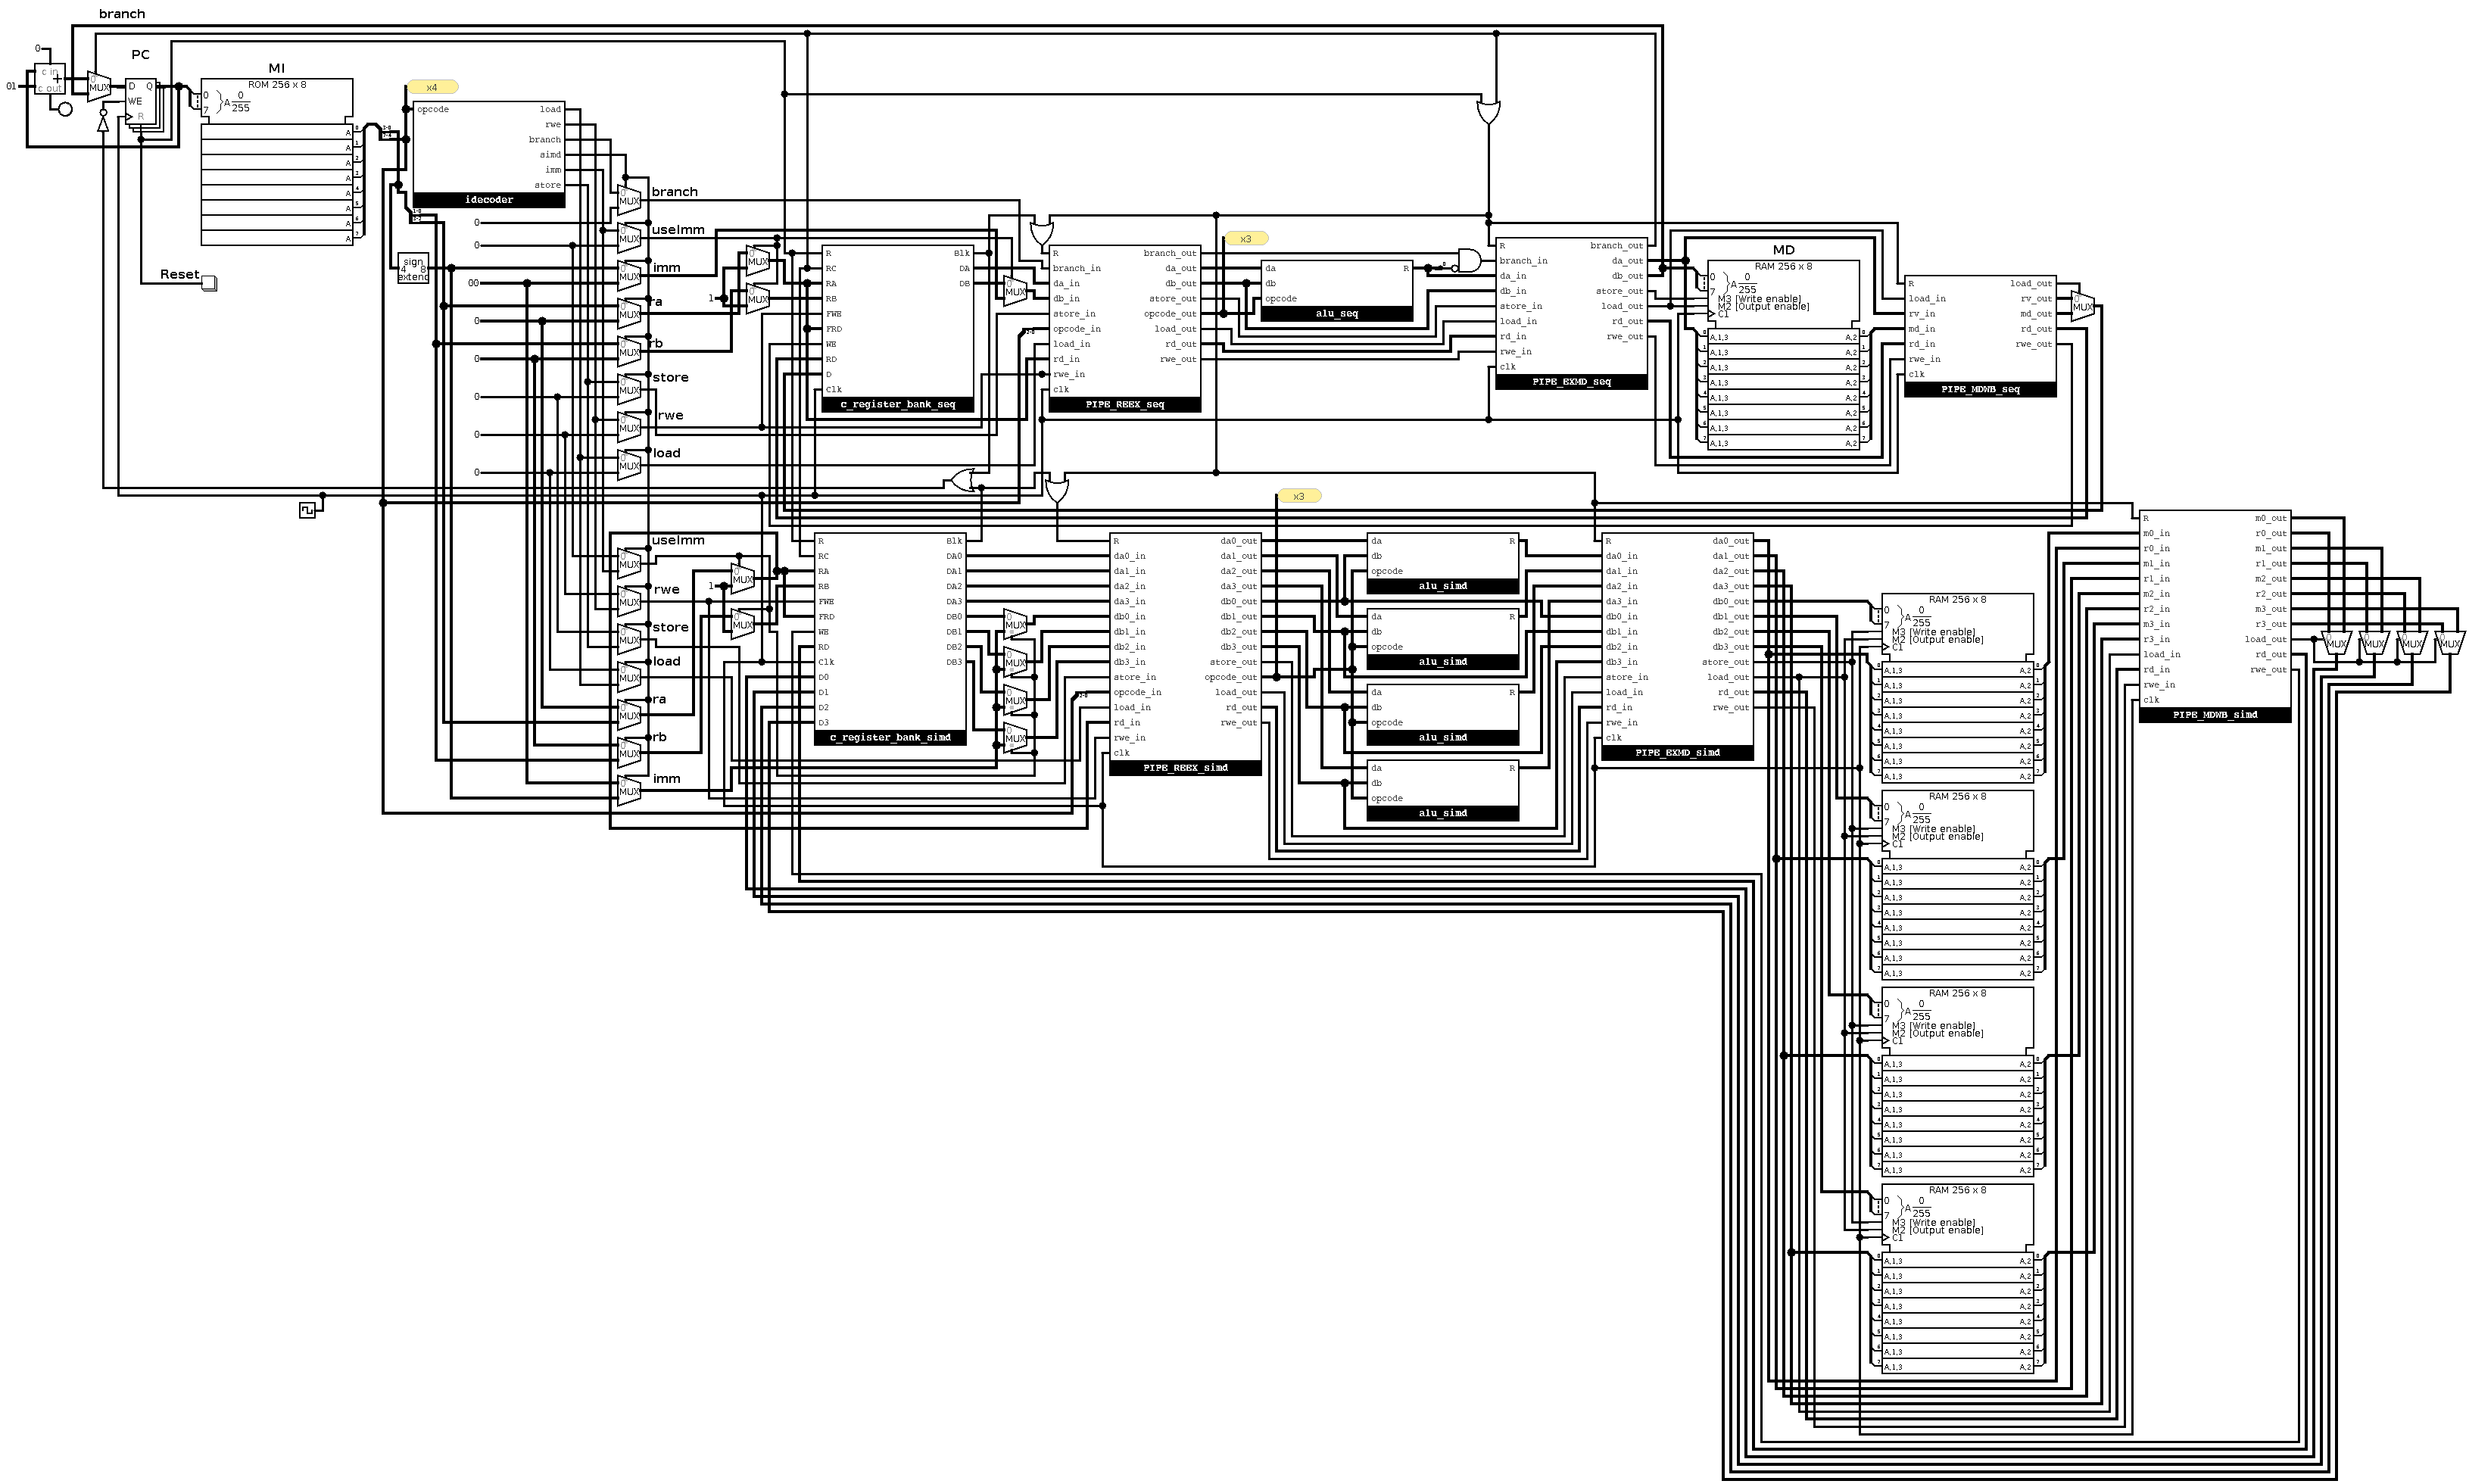
\includegraphics[width=0.9\textwidth]{main.png}
	\caption{Diagrama do Sagui em Bando.}
	\label{sagui}
\end{figure}

O circuito principal é semelhante ao circuito do Sagui \textit{pipeline}, porém
possui um segundo \textit{pipeline} acoplado. O módulo \textit{idecoder} foi
adaptado para a nova arquitetura, e um de seus sinais indica se a instrução é
do conjunto sequencial (caso em que o \textit{pipeline}) utilizado deve ser o
comum) ou do conjunto vetorial (caso em que o \textit{pipeline}) acoplado deve
ser utilizado. O outro, não utilizado na instrução atual, deve receber sinais
\textit{nop}.

O \textit{pipeline} acoplado agrega as unidades de processamento vetorial, sendo
4 no total. Elas dividem os estágios intermediários para sincronização, além de
utilizarem um mesmo banco de registradores (mostrado na seção \ref{banco}). Cada
unidade de processamento possui sua própria Unidade Lógica Aritmética e seu
próprio acesso à memória de dados.

A implementação possui memórias separadas para o \textit{pipeline} principal e
cada uma das unidades de processamento vetorial devido à limitações técnicas do
simulador e simplicidade de implementação. Isso não causou problemas na execução
dos programas de teste.

\section{A Unidade Lógica Aritmética}

A figura \ref{ula} apresenta o diagrama da Unidade Lógica Aritmética das
unidades de processamento vetorial.

\begin{figure}[h]
	\centering
	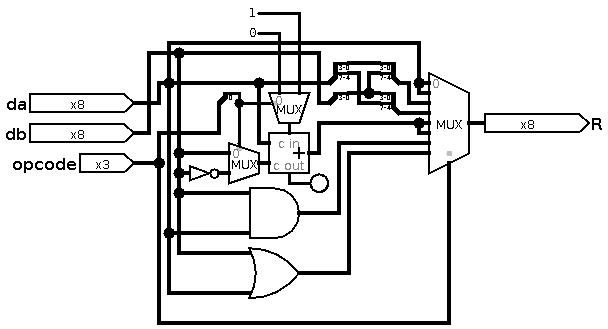
\includegraphics[width=\textwidth]{alu_simd.png}
	\caption{Diagrama da Unidade Aritmética da unidade de processamento vetorial
		do Sagui em Bando.}
	\label{ula}
\end{figure}

As unidades aritméticas utilizadas no Sagui comum, no \textit{pipeline}
principal do Sagui em Bando e em cada uma das unidades de processamento vetorial
são bem semelhantes, adaptadas para cada conjunto de instrução.

\section{O banco de registradores vetorial} \label{banco}

A figura \ref{fig-banco} mostra o diagrama do banco de registradores vetorial.

O banco de registradores do \textit{pipeline} vetorial é uma adaptação do banco
de registradores sequencial. Como cada unidade executa as mesmas instruções,
somente um contador para cada endereço de registrador é necessário. Além disso,
os registradores 0 foram substituídos pelas devidas constantes.

\begin{figure}[h]
	\centering
	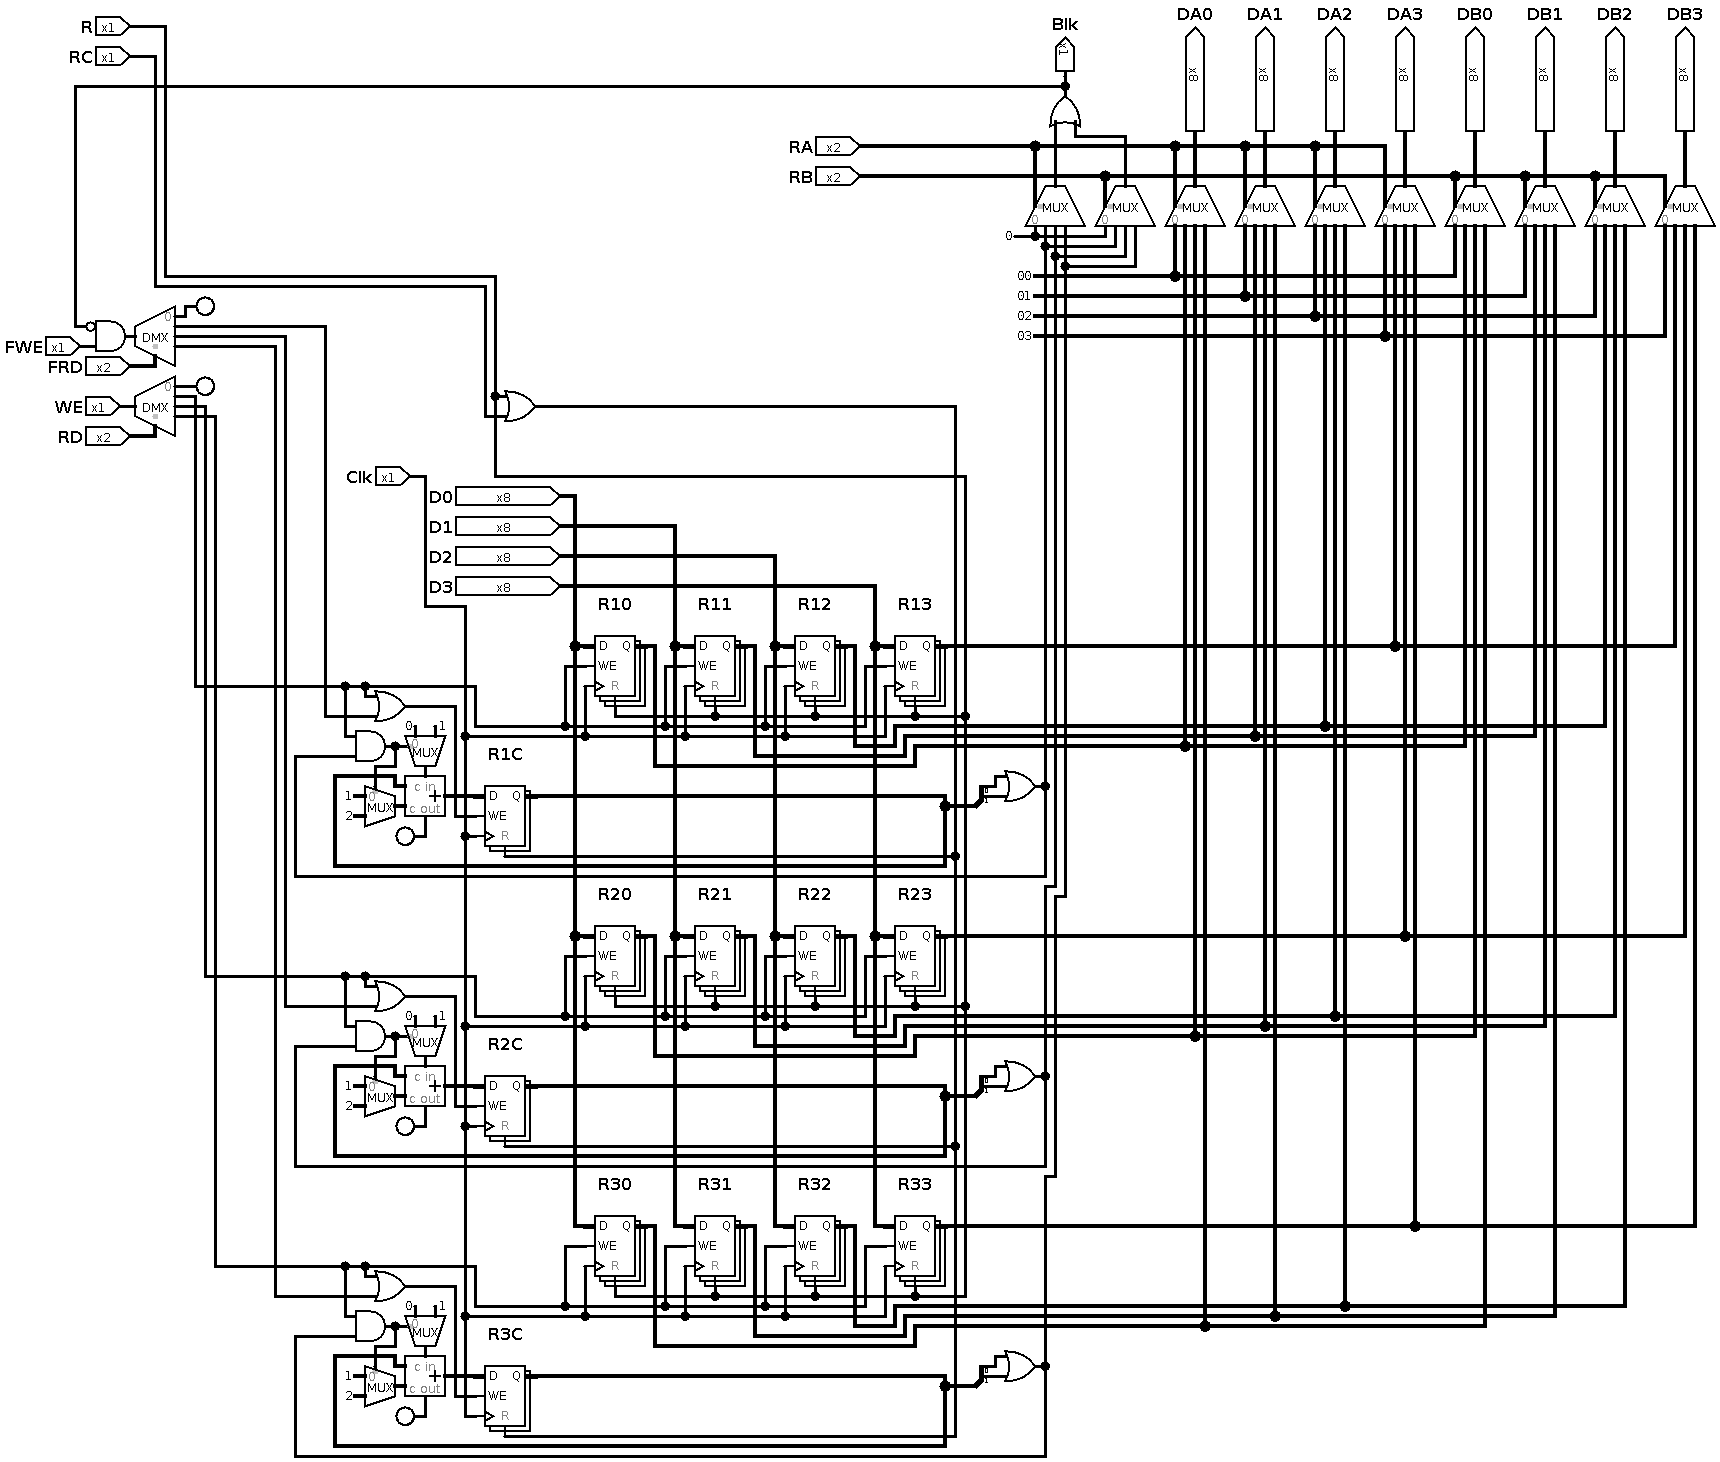
\includegraphics[width=\textwidth]{register_bank.png}
	\caption{Diagrama do banco de registradores vetorial.}
	\label{fig-banco}
\end{figure}

\section{Os programas de teste}

Foram desenvolvidos dois programas de teste para o processador. O primeiro
utiliza todas as instruções para averiguar o funcionamento correto:

\begin{verbatim}
; Teste das instruções.
; Para ser montado com o script saguisimdasm.exs.

; Zera todos os registradores.
sub r1, r1
sub r2, r2
sub r3, r3

movh 0xf
movl 0xa
; r1 deve ser 0xfa.

add r2, r1
; r2 deve ser 0xfa.

movh 0
sub r2, r1
; r2 deve ser 0xf0.

add r2, r1
; r2 deve ser 0xfa.

movl 0
movh 0xf
and r2, r1
; r2 deve ser 0xf0.

; Salto não deve ser tomado.
brzr r1, r3

; Salto deve ser tomado (instrução and deve ser pulada).
sub r2, r2
movl 0x2
movh 0x1
brzr r2, r1
and r0, r0

; Guarda o endereço 0 e valor 1 em r2 e r1 para o teste da memória.
movl 1
movh 0
sub r2, r2
st r1, r2
ld r3, r2
; r3 deve ser 1.

;
; Literalmente o mesmo teste porém vetorial.
;

v.sub r1, r1
v.sub r2, r2
v.sub r3, r3

v.movh 0xf
v.movl 0xa
; r1 deve ser 0xfa.

v.add r2, r1
; r2 deve ser 0xfa.

v.movh 0
v.sub r2, r1
; r2 deve ser 0xf0.

v.add r2, r1
; r2 deve ser 0xfa.

v.movl 0
v.movh 0xf
v.and r2, r1
; r2 deve ser 0xf0.
v.movl 0xa
v.or r2, r1
; r2 deve ser 0xfa novamente.

; Para a memória, somamos o endereço com o id do núcleo vetorial.
v.movl 1
v.movh 0
v.sub r2, r2
v.add r2, r0
v.st r1, r2
v.ld r3, r2
; r3 deve ser 1, e na memória deve ter [1,1,1,1] a partir do 0.
\end{verbatim}

O segundo realiza a soma de dois vetores:

\begin{verbatim}
; r1 -> jump target, tmp, etc
; r2 -> iterator
; v.r2 -> address
; v.r3 -> values

; load first array

v.sub r1, r1
v.sub r2, r2
v.sub r3, r3
v.add r2, r0
v.add r3, r0

sub r1, r1
sub r2, r2
movl 3
add r2, r1

;for:
movh 0x1
movl 0x6
brzr r2, r1

v.st r3, r2
v.sub r1, r1
v.movl 4
v.add r2, r1
v.add r3, r1

sub r1, r1
movl 1
sub r2, r1

movh 0x0
movl 0x9
brzr r0, r1
;endfor:

; load second array

v.sub r1, r1
v.sub r2, r2
v.sub r3, r3
v.add r2, r0
v.add r3, r0
v.movl 0xb
v.add r2, r1

sub r1, r1
sub r2, r2
movl 3
add r2, r1

;for:
movh 0x1
movl 0x6
brzr r2, r1

v.st r3, r2
v.sub r1, r1
v.movl 4
v.add r2, r1
v.add r3, r1

sub r1, r1
movl 1
sub r2, r1

movh 0x0
movl 0x9
brzr r0, r1
;endfor:

; zero third array

v.sub r1, r1
v.sub r2, r2
v.sub r3, r3
v.add r2, r0

v.movl 0x8
v.movh 0x1
v.add r2, r1

sub r1, r1
sub r2, r2
movl 3
add r2, r1

;for:
movh 0x1
movl 0x6
brzr r2, r1

v.st r3, r2
v.sub r1, r1
v.movl 4
v.add r2, r1

sub r1, r1
movl 1
sub r2, r1

movh 0x0
movl 0x9
brzr r0, r1
;endfor:

; finally sum everything "sequentially"

v.sub r1, r1
v.sub r2, r2
v.sub r3, r3
v.add r2, r1
v.add r3, r1
v.add r2, r0
v.add r3, r0
v.movl 12
v.add r3, r1
v.ld r3, r3
v.ld r1, r2
v.add r3, r1
v.movl 0x8
v.movh 0x1
v.add r2, r1
v.st r3, r2

v.sub r1, r1
v.sub r2, r2
v.sub r3, r3
v.add r2, r1
v.add r3, r1
v.add r2, r0
v.add r3, r0
v.movl 4
v.add r2, r1
v.movl 0
v.movh 0x1
v.add r3, r1
v.ld r3, r3
v.ld r1, r2
v.add r3, r1
v.movl 0x8
v.movh 0x1
v.add r2, r1
v.st r3, r2

v.sub r1, r1
v.sub r2, r2
v.sub r3, r3
v.add r2, r1
v.add r3, r1
v.add r2, r0
v.add r3, r0
v.movl 8
v.add r2, r1
v.movh 0x1
v.movl 0x4
v.add r3, r1
v.ld r3, r3
v.ld r1, r2
v.add r3, r1
v.movl 0x8
v.movh 0x1
v.add r2, r1
v.st r3, r2
\end{verbatim}

Para a montagem do Assembly, foi utilizado um script em linguagem
Elixir.\footnote{\url{https://elixir-lang.org/}}\footnote{Disponível em
	\url{https://gist.github.com/gboncoffee/1e2684405439e71384e4335032b0b74c}}

\end{document}
